\documentclass[12pt]{article}
\usepackage{sbc-template}
\usepackage{graphicx,url}
\usepackage[brazil]{babel} 
\usepackage[utf8]{inputenc}
\usepackage{placeins}
\usepackage{longtable}

\sloppy

\title{Plano de gerenciamento de riscos:\\Site de venda de ingressos para cinema}

\author{
    \begin{minipage}{\textwidth}
        Carlos\inst{1},
        Daniela Menezes\inst{1},
        Danilo\inst{1},
        Gabriel Augusto R. dos Reis\inst{1},
        Giovani\inst{1},
        Guilherme\inst{1},
        Indianara Santos Rodrigues\inst{1},
        Luiz\inst{1}
    \end{minipage}
}
\address{
    Departamento de Computação e Sistemas\\
    Universidade Federal de Ouro Preto (UFOP) -- João Monlevade, MG
}

\begin{document}

    \maketitle

    \begin{abstract}
        General overview of work.
    \end{abstract}
     
    \begin{resumo}
        Síntese geral do trabalho.
    \end{resumo}
    
    \section{Objetivo do Plano de gerenciamento de riscos}
        Este plano de gerenciamento tem como objetivo identificar todos os riscos associados ao projeto, assim como entendê-los afim de evitá-los e caso eles ocorram saber como corrigir a falha. A identificação e avaliação desses riscos serão realizadas em um brainstorming, além de utilizar a análise SWOT, detalhada na figura \ref{fig:swot}, assim como checklists e as lições aprendidas com projetos anteriores.
        \begin{figure}[h!]
                \centering
                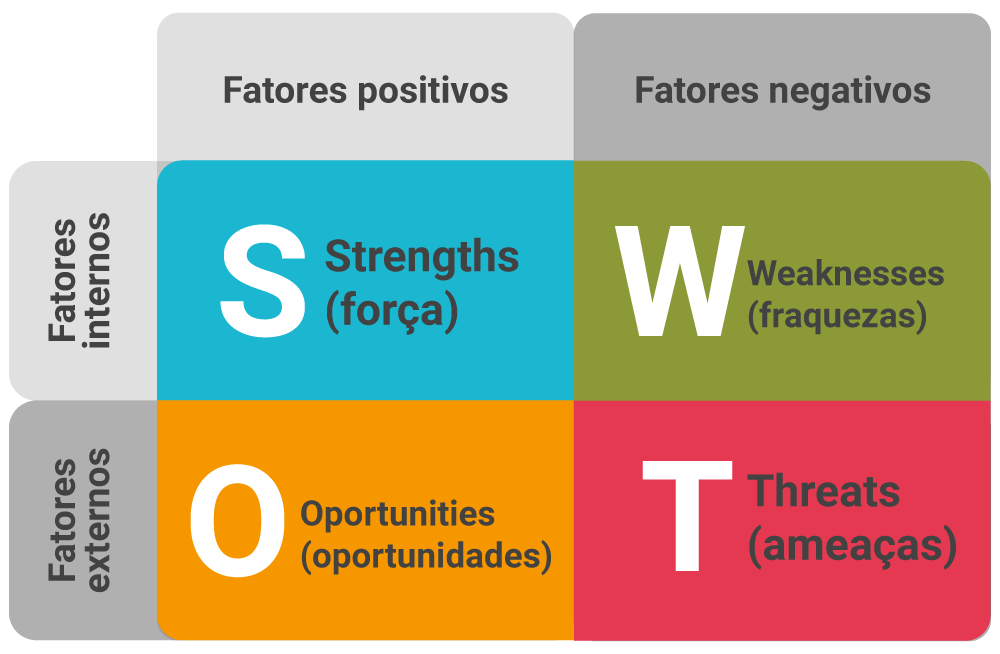
\includegraphics[scale=0.3]{./Images/swot.png}
                \caption{Gráfico SWOT}
                \label{fig:swot}
            \end{figure}

    \section{Identificar riscos associados ao projeto}
        \begin{itemize}
            \item Perda de dados.
            \item Layout ruim.
            \item Usabilidade confusa.
            \item Repostas erradas do Banco de dados.
            \item Erros de sincronização com os métodos de pagamento.
            \item Erros associados ao mecanismo de busca.
            \item Erros com editor de conteúdo.
            \item Erros relacionados a portabilidade.
            \item Número de usuários maior que o planejado.
            \item Usuários resistentes ao sistema.
            \item Ataque Hacker.
            \item Marketing ruim do site.
            \item Risco financeiro.
            \item Falta de atualização dos cinemas ou sessões.
            \item Preços não competitivos no mercado ou com o próprio cinema localmente.
            \item Satisfação do cliente. 
            \item Inutilização dos cinemas.
        \end{itemize} 
        
    \section{Avaliar probabilidade de ocorrência}
        De acordo com a Figura \ref{fig:swot}, os riscos identificados serão qualificados de acordo com sua probabilidade de ocorrência.
        
        \begin{itemize}
            \item  Probabilidade:
            \begin{itemize}
                \item Baixa - A probabilidade de ocorrência do risco pode ser considerada pequena.               
                \item Média - Existe uma probabilidade razoável de ocorrer o risco.
                \item Alta - O risco é iminente.
            \end{itemize}
            \item Gravidade:
            \begin{itemize}
                \item Baixa - O impacto do evento de risco é irrelevante, tanto em termos de custo, prazo, podendo ser resolvido facilmente.
                \item Média - O impacto de evento de risco é relevante e necessita de gerenciamento mais preciso.
                \item Alta - O impacto do evento de risco é elevado e, caso não haja uma interferência imediata e precisa, os resultados serão comprometidos.
            \end{itemize}
        \end{itemize}
       
        \begin{table}[h]
            \centering
            \label{table:gravidade_e_riscos}
            \resizebox{\textwidth}{!}{
                \begin{tabular}{|l|c|c|}
                    \hline
                    \multicolumn{1}{|c|}{\textbf{Riscos}} & 
                    \multicolumn{1}{|c|}{\textbf{Probabilidade}} & 
                    \multicolumn{1}{|c|}{\textbf{Gravidade}} \\ \hline
                    Perda de dados & baixa & alta \\ \hline
                    Layout ruim & baixa & baixa \\ \hline
                    Usabilidade confusa & baixa & média \\ \hline
                    Repostas erradas do Banco de dados & baixa & alta \\ \hline
                    Métodos de pagamento & baixa & alta \\ \hline
                    Mecanismo de busca & média & baixa \\ \hline
                    Portabilidade & média & alta \\ \hline
                    Número de usuários maior que o planejado & baixa & baixa \\ \hline
                    Ataque Hacker & média & alta \\ \hline
                    Marketing ruim do site & média & baixa \\ \hline
                    Risco financeiro & baixa & alta \\ \hline
                    Falta de atualização dos cinemas ou sessões & alta & alta \\ \hline
                    Preços não competitivos no mercado ou com o próprio cinema localmente & alta & alta \\ \hline
                    Satisfação do cliente & baixa & média \\ \hline
                    Inutilização dos cinemas & baixa & alta \\ \hline
                \end{tabular}
            }
            \caption{Probabilidade e gravidade dos riscos}
        \end{table}
    \FloatBarrier

    \section{Estimar impacto}

        \begin{center}
            \begin{longtable}{|p{2.0cm}|p{3.2cm}|c|p{3.2cm}|c|}
                
            
                \hline 
                \multicolumn{1}{|c|}{\textbf{Riscos}} & 
                \multicolumn{1}{c|}{\textbf{Descrição}} & 
                \multicolumn{1}{c|}{\textbf{Probabilidade}} &
                \multicolumn{1}{c|}{\textbf{Impacto}} &
                \multicolumn{1}{c|}{\textbf{Gravidade}} \\ \hline 
                \endfirsthead

                \multicolumn{5}{c}%
                {{\bfseries \tablename\ \thetable{} -- continuação da última página}} \\
                \hline 
                \multicolumn{1}{|c|}{\textbf{Riscos}} & 
                \multicolumn{1}{c|}{\textbf{Descrição}} & 
                \multicolumn{1}{c|}{\textbf{Probabilidade}} &
                \multicolumn{1}{c|}{\textbf{Impacto}} &
                \multicolumn{1}{c|}{\textbf{Gravidade}}\\ 
                \endhead

                \hline 
                \multicolumn{5}{|r|}{{Continua na próxima página}} \\ \hline
                \endfoot

                \hline \hline
                \endlastfoot
                
                Perda de dados & Devido a problemas no banco de dados, os dados podem ser momentaneamente perdidos & baixa & O software pode ficar inoperante até que o problema seja resolvido. & alta \\ \hline
                
                Layout ruim & Caso o site não funcione corretamente não irá proporcionar uma experiência agradável ao usuário  & baixa  & Perda de usuários e consequentemente perda de lucro & baixa  \\ \hline
                
                Usabilidade confusa & Uma navegação complexa pode fazer com que o visitante abandone o site. & baixa  & Perda de visitantes & média \\ \hline
                
                Repostas erradas do Banco de dados & Banco de dados retornam ingressos ou dados relativos ao ingressos ou sessões de forma errada & baixa & Gera compras erradas, inesperadas ou inexistentes, causando transtorno aos clientes, prejuízo ao site e má reputação perante os clientes & alta  \\ \hline
                
                Métodos de pagamento & Método de pagamento para de responder como o esperado, deixando de efetuar ou confirmar as transações & baixa & Parada nas vendas, gerando prejuízos até que o sistema retorne ao normal & alta  \\ \hline
                
                Mecanismo de busca & Campos de busca são áreas bastante utilizadas para encontrar o conteúdo do site o mais rápido possível. & média  & Visitante frustrado e consequentemente perda de visitantes  & baixa  \\ \hline
                
                Portabilidade & Site funciona de forma inesperada em browsers ou dispositivos diferentes & média & Usabilidade ruim do site & alta \\ \hline
                
                Número de usuários maior que o planejado & Número de usuários acessando simultaneamente o site é maior que o esperado & baixa & Clientes ativos não terão problemas, a medida que os novos visitantes não conseguirão acessar até que um antigo saia e libere o recurso & baixa \\ \hline
                
                Ataque Hacker & Devido a uma falha de segurança em qualquer parte da infraestrutura, uma pessoa mal-intencionada, pode invadir o servidor e ter acesso a dados privados, podendo alterá-los ou divulgá-los de forma indevida. & média & A empresa pode sofrer processos legais caso os dados privados sejam descobertos ou o site pode ficar temporariamente inoperante. & alta \\ \hline 
                
                Marketing ruim do site & divulgação de forma errada, sem alcance ou desinteressante aos possíveis clientes & média & Desinteresse de novos clientes & baixa  \\ \hline
                
                Risco financeiro & Incerteza sobre futuro financeiro da empresa & baixa & Revisão nos planos da empresa & alta  \\ \hline 
                
                Falta de atualização dos cinemas ou sessões & Não atualizar os dados dos cinemas ou sessões de filmes & alta & Compras erradas ou falta de opções de compra & alta  \\ \hline 
                
                Preços não competitivos no mercado ou com o próprio cinema localmente & Preços mais caros ou não vantajosos quando comparado com concorrentes ou o próprio cinema & alta & Não serão realizadas novas vendas & alta  \\ \hline 
                
                Satisfação do cliente & reclamações sobre o site, principalmente nas redes sociais & baixa & danos à identidade digital & média  \\ \hline 
                
                Inutilização dos cinemas & Tecnologia ficar ultrapassada ou ser substituída & baixa & Adequação ao novo mercado ou tecnologia & alta  \\ \hline 
              
                \caption{Descrição dos riscos e seus Impactos}
                \label{Descricao_E_Impacto_Dos_Riscos}
            \end{longtable}
        \end{center}

        
    \subsection{Estabelecer plano de contingência}
       
       \begin{itemize}
       \item Perda de dados: A melhor forma de evitar a perda de dados é fazer backups periódicos ou sistemas distribuídos.
       
       \item  Layout ruim: Para que o site funcione corretamente e proporcione uma experiência agradável ao usuário é necessário que a parte visual/estética estejam alinhados. Caso haja exagero nas cores, tamanho de imagem inadequado que atrapalhe a qualidade visual da tela é necessário que o layout seja refeito.
       
        \item Usabilidade confusa: É necessário que parte do site seja refeito de maneira simples, inidentificável e direta, seguindo o padrão na construção das páginas, agrupar o conteúdo do site em categorias lógicas fazendo com que a resposta por uma procura seja mais direta possível.
        
        \item Respostas erradas do banco de dados: Caso seja identificado um método de pequisa que gere uma resposta errada, um desenvolvedor de manutenção do software deve ser chamado para que posso ser analisado o motivo do erro e então liberada uma versão de correção do software o mais rápido possível.
        
        \item Métodos de pagamento: Contactar imediatamente a empresa terceirizada responsável pelo pagamento para que seja reparado ou se necessário, efetuar a troca da empresa terceirizada.
       
        \item Mecanismo de busca: Caso as buscas gerem resultados inesperados, as consultas feitas no banco de dados devem ser repensadas para que os erros não se repitam.
        
        \item Portabilidade: Caso seja identificado um dispositivo ou browser que gere um layout     método de pequisa que gere um layout "quebrado", deve-se verificar quais as características do dispositivo para que possa ser corrigido e então liberar uma versão de correção do software o mais rápido possível.
        
        \item Número de usuários maior  que o planejado: Caso o site não suporte a quantidade de usuários, será necessário aumentar a capacidade do servidor.
        
        \item  Ataque Hacker: Verificar em qual área o ataque foi feito, caso sejam dados privados, alertar a todos os envolvidos imediatamente, caso dados sejam modificados, o backup deverá ser consultado e restaurado, caso contrário reestabelecer o servidor para que o site volte a operar normalmente.
        
        \item Marketing ruim do site: Após verificar a efetividade do marketing atual (cruto, médio e longo prazo), refazer todo o conceito de divulgação do site.
        
        \item Risco financeiro:  Revisão constante das finanças e planejamento financeiro futuro detalhado e discutido com os administradores da empresa.
        
        \item Falta de atualização dos cinemas ou sessões: contratar novo funcionário para tal função ou integrar banco de dados do site com o do cinema.
        
        \item Preços não competitivos no mercado ou com o próprio cinema localmente: Revisão na metodologia financeira da empresa, afim de diminuir os preços.
        
        \item Satisfação do cliente: Para evitar esse risco, um SAC (Serviço de Atendimento ao Consumidor) precisa ser colocado em prática na estratégia de marketing digital. Reclamações de qualquer natureza devem ser respondidas.
        
         \item Inutilização dos cinemas: Adequação a nova tecnologia existente e/ou mercado.
        
       \end{itemize}

    \section{Riscos de projeto}
        Os riscos de projeto estão relacionados com aspectos operacionais, organizacionais e contratuais, que são de responsabilidade do Gerente do Projeto. Em sua descrição está incluído o relacionamento com os fornecedores, restrições contratuais, interfaces externas, requisitos, clientes, organização e limitações de recursos a serem utilizados. Tais riscos ameaçam diretamente o plano do projeto, podendo vir a atrasar o cronograma e também elevar os custos do mesmo, uma vez que o maior risco dos projetos de software é o financeiro pois, a obtenção de recursos orçamentários pode variar de acordo com o mercado financeiro, por exemplo.
    \section{Riscos técnicos}
        Carlos
    \section{Riscos de negócio}
        Giovani
    \section{Risco de marketing}
        O marketing é uma grande aliado para empresa, pois ele otimiza o lucro da empresa através da oferta de mercadorias ou serviços de acordo com a necessidade e preferência dos consumidores. 
        O marketing pode ser realizado através de propagandas, pesquisas de mercado, design, entre outras. 
        Com o objetivo de saber como anda a questão do marketing de vendas de ingressos de cinema, fizemos pesquisa com algumas pessoas para saber se elas têm acesso a publicidade envolvendo a venda de ingressos. Bom, a pesquisa tão teve um resultado bom como podemos ver na tabela\ref{table:freq_divulgacao}.
        
      \begin{table}[h]
            \centering
            \resizebox{\textwidth}{!}{
                \begin{tabular}{|c|c|c|c|c|c|c|c|c|c|c|c|}
                    \hline
                    \multicolumn{1}{|c|}{\textbf{}} & 
                    \multicolumn{1}{c|}{\textbf{Carlos}} & 
                    \multicolumn{1}{c|}{\textbf{Danilo}} & 
                    \multicolumn{1}{c|}{\textbf{Gabriel}} & 
                    \multicolumn{1}{c|}{\textbf{Giovani}} & 
                    \multicolumn{1}{c|}{\textbf{Giovanna}} & 
                    \multicolumn{1}{c|}{\textbf{Guilherme}} & 
                    \multicolumn{1}{c|}{\textbf{Indianara}} &
                    \multicolumn{1}{c|}{\textbf{Luiz}} &
                    \multicolumn{1}{c|}{\textbf{Micael}} &
                    \multicolumn{1}{c|}{\textbf{Nicole}} &
                    \multicolumn{1}{c|}{\textbf{Vanessa}} \\ \hline
                    Frequentemente & & & & & & & & & & & \\ \hline
                    Raramente & X & X & X & X & X & X & X & X & & X & X \\ \hline
                    Nunca & & & & & & & & & X & & \\ \hline
                \end{tabular}
            }
            \caption{Com que frequência você vê divulgações de vendas de ingressos?}
            \label{table:freq_divulgacao}
        \end{table}
        \FloatBarrier
        
    É preocupante nos dias de hoje que não haja propaganda frequente sobre um determinado produto, visto que há grande procura de informações na internet sobre cinema e venda de ingressos visto na \ref{table:Meio_de_obter_info}, pois é uma maneira ágil e prática para a maiorias das pessoas. Se houvesse mais divulgação talvez não seria tão necessária a busca do cliente nos sites, mas sim já apareceria aquilo que o interessa fazendo que ele compre sempre e não só quando lança algum filme imperdível.
    
    \begin{table}[h]
            \centering
            \resizebox{\textwidth}{!}{
                \begin{tabular}{|c|c|c|c|c|c|c|c|c|c|c|c|}
                    \hline
                    \multicolumn{1}{|c|}{\textbf{}} & 
                    \multicolumn{1}{c|}{\textbf{Carlos}} & 
                    \multicolumn{1}{c|}{\textbf{Danilo}} & 
                    \multicolumn{1}{c|}{\textbf{Gabriel}} & 
                    \multicolumn{1}{c|}{\textbf{Giovani}} & 
                    \multicolumn{1}{c|}{\textbf{Giovanna}} & 
                    \multicolumn{1}{c|}{\textbf{Guilherme}} & 
                    \multicolumn{1}{c|}{\textbf{Indianara}} &
                    \multicolumn{1}{c|}{\textbf{Luiz}} &
                    \multicolumn{1}{c|}{\textbf{Micael}} &
                    \multicolumn{1}{c|}{\textbf{Nicole}} &
                    \multicolumn{1}{c|}{\textbf{Vanessa}} \\ \hline
                    Aplicativos & & & & & & & & & & & \\ \hline
                    Sites & X & X & X & X & X & X & X & X & X & X & X \\ \hline
                    Cartazes & & & & & & & & &  & & \\ \hline
                \end{tabular}
            }
            \caption{Na hora de escolher o filme para qual você irá comprar ingressos, qual meio você procura para obter informações?}
            \label{table:Meio_de_obter_info}
        \end{table}
        \FloatBarrier
    
    Um ponto positivo é que das pessoas que viram alguma publicidade disseram que essas publicidades tinham a ver com seu gostos.

      \begin{table}[h]
            \centering
            \resizebox{\textwidth}{!}{
                \begin{tabular}{|c|c|c|c|c|c|c|c|c|c|c|c|}
                    \hline
                    \multicolumn{1}{|c|}{\textbf{}} & 
                    \multicolumn{1}{c|}{\textbf{Carlos}} & 
                    \multicolumn{1}{c|}{\textbf{Danilo}} & 
                    \multicolumn{1}{c|}{\textbf{Gabriel}} & 
                    \multicolumn{1}{c|}{\textbf{Giovani}} & 
                    \multicolumn{1}{c|}{\textbf{Giovanna}} & 
                    \multicolumn{1}{c|}{\textbf{Guilherme}} & 
                    \multicolumn{1}{c|}{\textbf{Indianara}} &
                    \multicolumn{1}{c|}{\textbf{Luiz}} &
                    \multicolumn{1}{c|}{\textbf{Micael}} &
                    \multicolumn{1}{c|}{\textbf{Nicole}} &
                    \multicolumn{1}{c|}{\textbf{Vanessa}} \\ \hline
                    Sim & X & X & X & & & X & X & X & X & X & X \\ \hline
                    Não & & & & X & X & & & & & & \\ \hline
                \end{tabular}
            }
            \caption{Propagandas de vendas de ingressos geralmente estão relacionadas com seu gosto?}
            \label{table:Propagandas_ao_gosto}
        \end{table}
        \FloatBarrier
    Por fim, vimos que o marketing de vendas de ingressos de cinema é fraco entre as pessoas entrevistadas, e que com certeza o mercado poderia lucrar mais se houvesse mais divulgação. Por mais que a indústria do cinema se garanta e não entre em decadência, por sempre fazer as estreias do filme, o marketing responsável otimizar esse processo adquirindo sempre novos clientes e mantendo os que já tem.

    
    \section{Risco gerencial}
        Giovani
        
    \section{Risco orçamentário}
        Vários riscos podem comprometer o andamento de um projeto, inclusive o orçamentário.
        Atraso no cronograma de desenvolvimento de um site de venda de ingresso pode causar custos maiores que o previsto. O fatores que geram esse prejuízo são, aumento de gastos com a empresa que desenvolve o software e enquanto mais demora a ficar pronto um site de vendas, maior é tempo que essa empresa não vende pela internet, sendo que nos dias de hoje muitos dos consumidores preferem a praticidade e agilidade de comprar pela internet.
        Manutenção, novas tecnologias também geram custos para empresa que deve estar sempre preparadas para essas situações.
        Depois que temos um site de vendas de ingresso de cinema pronto e funcionando corretamente é necessário alavancar as vendas através do marketing, mostrando para o público aquilo que ele quer ver de acordo com suas preferências, visto que em uma pesquisa feita a maioria das pessoas preferem assistir filme no cinema de acordo com a tabela \ref{table:preferencia_local_ver_filme}.
    
          \begin{table}[h]
            \centering
            \resizebox{\textwidth}{!}{
                \begin{tabular}{|c|c|c|c|c|c|c|c|c|c|c|c|}
                    \hline
                    \multicolumn{1}{|c|}{\textbf{}} & 
                    \multicolumn{1}{c|}{\textbf{Carlos}} & 
                    \multicolumn{1}{c|}{\textbf{Danilo}} & 
                    \multicolumn{1}{c|}{\textbf{Gabriel}} & 
                    \multicolumn{1}{c|}{\textbf{Giovani}} & 
                    \multicolumn{1}{c|}{\textbf{Giovanna}} & 
                    \multicolumn{1}{c|}{\textbf{Guilherme}} & 
                    \multicolumn{1}{c|}{\textbf{Indianara}} &
                    \multicolumn{1}{c|}{\textbf{Luiz}} &
                    \multicolumn{1}{c|}{\textbf{Micael}} &
                    \multicolumn{1}{c|}{\textbf{Nicole}} &
                    \multicolumn{1}{c|}{\textbf{Vanessa}} \\ \hline
                    Em casa & & X & & & & & X & & X & X & X \\ \hline
                    No cinema & & & X & X & X & X & & X & & & \\ \hline
                \end{tabular}
            }
            \caption{Preferência de local para ver filme}
            \label{table:preferencia_local_ver_filme}
        \end{table}
        \FloatBarrier
    
    Então o risco orçamentário pode ser visto de dois modos, como perda de dinheiro com gastos na hora de planejar um site e a perda de vendas que poderiam ser alcançadas através da publicidade.
    No fim de todo o processo do desenvolvimento do software é necessário que ele atenda todas as necessidades dos clientes e que esse site chegue ao maior número de pessoas possíveis.


    \section{Mitigação}
        Guilherme
    \section{Monitoramento}
        ??????????????
    \section{Gerência de riscos}
        ??????????????
    \section{Conclusão}
        ??????????????

    \nocite{*}
    \bibliographystyle{IEEEtran}
    \bibliography{sbc-template}
\end{document}